\documentclass[master.tex]{subfiles}
 
\begin{document}


\section{Structural Overview}
The execution contains three distinct steps where the last two run in parallel. At first the simulation must be initialized using a provided parameters file or restarting from previous data. Afterwards the actual simulation starts. In this context a single iteration contains these steps:
\begin{enumerate}
    \item Execute gyroaveraging for ion species (\autoref{sec:components-gryoaverage})
    \item Apply external sources and boundaries (\autoref{sec:components-external})
    \item Solve polarization equation (\autoref{sec:components-polarization})
    \item Update global variables (current $\mathrm{J})$
    \item Calculate right hand side of model equations
    \item Calculate new time step for each equation
    \item Update derived quantities
\end{enumerate}
Depending on the parameters data output steps are performed. This is not done every iteration to save computation speed since input output operations are typically slow.
\begin{enumerate}
    \item Every 20 iterations calculate combined quantities (Turbulent Flow...)
    \item Write data to hard drive depending on current iteration and parameters
\end{enumerate}
\section{Components}
\subsection{Initialization}
\subsubsection{Fresh start}
At first the parameter file is read and parameters and domain objects containing all information about the simulation and grid are created. From these objects all other objects are constructed and the necessary memory is allocated.\\
Following the electron density is initialized using the method \textit{Init::initCloseToData2} that essentially creates a differentiable profile:
\begin{figure}[!hbt]
    \centering
    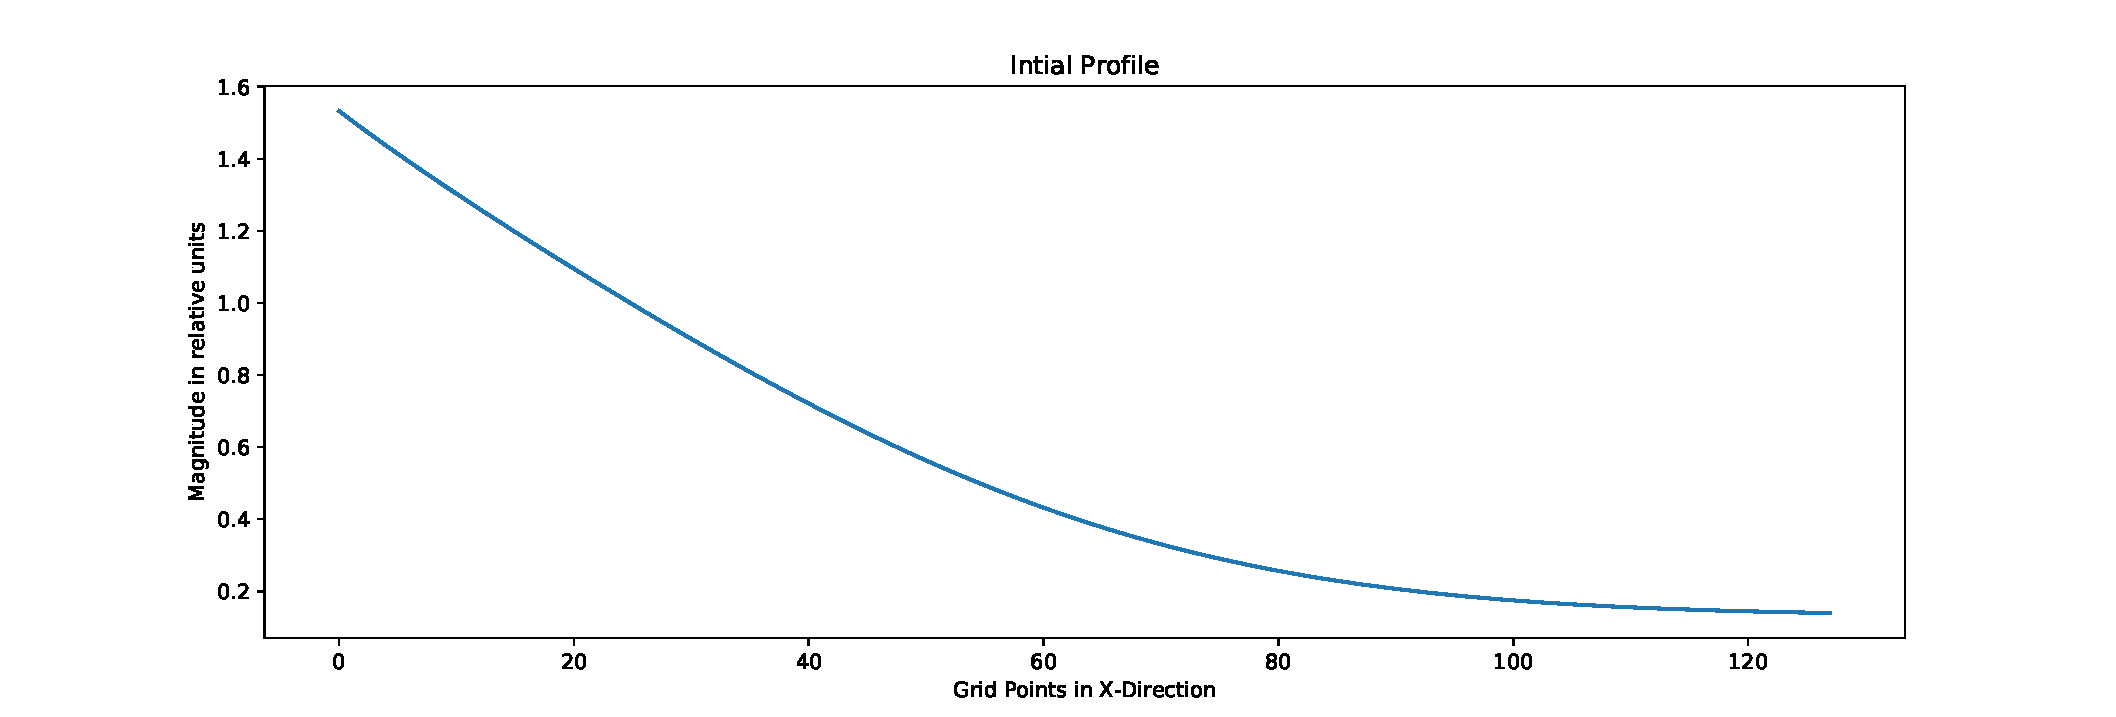
\includegraphics[width=\linewidth]{pdfs/initial_profile.pdf}
    \caption{Initial profile from initial electron and ion density is derived.}
    \label{fig:initial_profile}
\end{figure}

This data is saved as background profile to have a reference later on.
Then some fluctuations are added in the core plasma to trigger turbulence (\textit{Init::initTurbulentBath}). Afterwards the ion density is initialized:
\begin{equation}
    n_i = n_e - \frac{\tau_i \mu_i}{2} \Delta n_e
\end{equation}
This further \textit{seeds} the turbulence. The last thing to do is to set the previous time steps of the time iterators to the current value. These are considered our initial values:
\begin{equation}
    \xi^{(-i)} = \xi_{init} \colon i = 0, 1, 2
\end{equation}


\subsubsection{Restart}
On a restart the only necessary step is to initialize the time stepper since the previous steps are not stored in the data file. This creates a small error that most likely only has a small effect on the data if the simulation runs for a sufficient time afterwards but has not been evaluated properly and should be avoided. A solution would be to also save data of the previous steps.

\subsection{Gyroaveraging of Ions {\small "src/models/isothermal/gyroaveraging.cpp"}}
\label{sec:components-gryoaverage}
The work consists of applying the transformation from \autoref{eq:gyro-transformation} and then doing two Fourier transformation. Finally the result is written back. This is done in \textit{Poisson::fftwSolver2D} in file \textit{"src/algorithms/poisson/fftwsolver.cpp"}.
A second implementation is available executing the code on the GPU using the \textit{cufft}-library from the nvidia cuda toolkit. The steps are shown in \autoref{eq:gyroaveraging-steps}. The non fourier transformation is always done on the CPU but the fourier transformation may either be executed on the CPU or the GPU.

\begin{equation}\label{eq:gyroaveraging-steps}
    \begin{split}
    &n \overset{t}{\longrightarrow} n_t \overset{DFT}{\longrightarrow} \mathcal{F}(n_t)\\
    &\mathcal{F}(n_t) \overset{\cdot C_i}{\longrightarrow} \mathcal{F}(N_t)\\
    &\mathcal{F}(N_t) \overset{DFT^{-1}}{\longrightarrow} N_t \overset{t^{-1}}{\longrightarrow} N
    \end{split}
\end{equation}

\subsection{External Sources {\small "src/models/isothermal/external3d.cpp"}}
\label{sec:components-external}
This step is necessary to keep the simulation stable at the edges. There is a zone on the left and on the right x-boundary. The borders of the zone are smoothed out to prevent high gradients. At first the gyroaveraged density of the ions is forced to the background density. Afterwards $\Gamma_0^{-1}$ is applied and the other densities are forced to equal this inverse:

\begin{align}
    N_i &= (N_i - n_0) \cdot \alpha(x) + n_0\\
    n_e &= (n_e - \Gamma_1^{-1}N_i) \cdot \alpha(x) + \Gamma_1^{-1}N_i\\
    n_i &= (n_i - \Gamma_1^{-1}N_i) \cdot \alpha(x) + \Gamma_1^{-1}N_i
\end{align}
 \todo{Chart of $\alpha(x)$}
 
 \subsection{Polarization Equation {\small "src/models/isothermal/polarization3d.cpp"}}
\label{sec:components-polarization}
The code execution is straight forward.
\begin{enumerate}
    \item Calculate right hand side ($F$) and non-linearity ($N$) of: $\nabla N \nabla \phi = F$
    \item Choose initial values of solver to be: $\phi_0 = \phi^{-1} + 0.75 \cdot (\phi^{-1} - \phi^{-2})$
    \item Execute solver (either on CPU or GPU) (\autoref{sec:sor-solver-implementation})
    \item Calculate gyro-screen potential
    \item Add a special non-linear term which is not discussed here
    \item Update potential ghost cells where necessary
\end{enumerate}


\section{SOR-Solver Implementation}
\label{sec:sor-solver-implementation}
There are two different implementations available. Both solve \autoref{eq:general-nonlinear-poisson} on a 2-dimensional grid.
\begin{equation}
    \nabla N(x,y)\nabla U(x,y) = F(x,y)\label{eq:general-nonlinear-poisson}
\end{equation}
Specific boundary conditions are employed:
\begin{equation}
    \begin{split}
        U(x, 0) &= U(x, n_y - 1) \\
        U(x, n_y) &= U(x, 1)\\
        U(0, y) &= 0\\
        U(n_x, y) &= U(n_x - 1, y)
    \end{split}
\end{equation}
Formulated in words this means that the domain is circular in y-direction, Dirichlet bound in the left-x direction and open ended in the right-x direction.
The implementation uses a Red-Black iteration scheme which allows to always use the newest data points and thus increases convergences. The algorithm first builds a linear system of equations by discretization of the non linear Poisson equation (\autoref{sec:polarization-equation}). The resulting equation
\begin{equation*}
    AU = F
\end{equation*}
is then solved using the \ac{SOR} \cite{SORPaper} method.

\subsubsection{CPU Implementation}
On the CPU the red black scheme is implemented by two sweeps over the complete matrices. The inner loop over the y dimension is vectorized by the compiler. The implementation is straight forward and easy to understand.

\subsubsection{GPU Implementation}
On the GPU a different approach has been taken. Since it is faster to load adjacent data points into shared memory (coalesced memory access) it is useful to rearrange the data and split them into two matrices. One containing all the red (even) data points and the other all black (odd) data points. The implementation follows the one presented in this conference article \cite{CUDARedBlack}.

\section{Modularization}
A moderately high level of abstraction is employed in the code base to allow modularization. In this context this means that specific parts of the code are easily interchangeable with newer/other implementations. To make this possible the components may only be loosely coupled. \autoref{fig:highLevelCodeStructure} shows the general structure of the code. Now it can easily be seen that the implementation of a new model can simply reuse \textit{Algorithms, Domain and Core} modules of the existing models. Furthermore one can for example improve the algorithms without greater knowledge about the model since the algorithms do not depend on the models. Also the implementation of newer models does not interfere with the function of the existing models.
\begin{figure}[h]
    \centering
    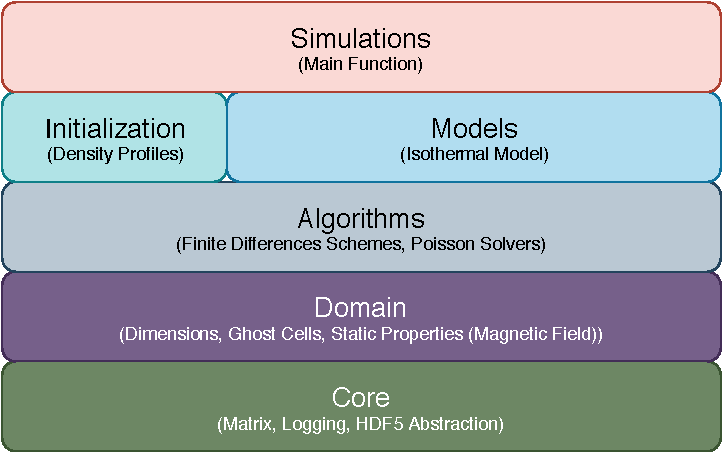
\includegraphics[]{pdfs/code_modules_high_level.pdf}
    \caption{High level structure of code. Each module may only depend on all beneath it.}
    \label{fig:highLevelCodeStructure}
\end{figure}

\section{Input}
The simulation parameters are provided via a \ac{JSON} configuration file. The default file name is \textit{"config.json"} but one may specify another file using the \textit{"-c <config-file>"} command line option. The available parameters are described in the wiki of the repository (\href{https://git.uibk.ac.at/csat8630/t3g-cmake/wikis/parameters}{Link-Wiki-Repository}). It is also possible to restart computation from a data file using \textit{"-r <data-file>"}. This restarts from the last saved iteration. One may also provide a specific data set to restart from using \textit{"-s <iteration-number>"}. For Example:
\begin{quote}
    \small
./Isothermal3d -r "\url{~/data/specialRun.hdf5}" -s 10001
\end{quote}
or even restart with new parameters:
\begin{quote}
\small
      ./Isothermal3d -c "\url{~/configs/specialRun2.json}" -r "\url{~/data/specialRun.hdf5}" -s 10001  
\end{quote}
A running simulation can not be changed though this may be implemented quite easily.

\section{Output}
\label{sec:output}
The output is collected into a single \ac{HDF5} file. The structure for the Isothermal model simulation is discribed here \textit{\href{https://git.uibk.ac.at/csat8630/t3g-cmake/wikis/Isothermal/Output}{Wiki Isothermal Output}}.

\section{Python Plotter}
The repository contains a small python application to visualize data. It uses \textit{PyQt5} and \textit{matplotlib}. It is found in the folder \textit{"plotter"} and can be started using
\begin{quote}
    python main.py
\end{quote}
in a suitable environment. The application creates 2D heatmaps of the densities, parallel velocities, potential and vorticity as well as radial profiles. Further more it can plot the energetics output.

\end{document}